\documentclass[12pt]{article}
\usepackage{graphicx} % Required for inserting images
\usepackage{enumitem}
\usepackage{amsmath}
\usepackage{gvv-book}
\usepackage{gvv}

\title{\textbf{4.2.8}}
\author{\textbf{EE25BTECH11005 - Aditya Mishra}}
\date{September 20, 2025}

\begin{document}

\maketitle

\section*{Question}
Find the direction and normal vectors of the line $5 = 2x$.

\section*{Solution}

The equation of the line can be written as
\begin{align}
2x - 5 = 0
\end{align}

The slope of the line $x = \frac{5}{2}$ is undefined, therefore it can be expressed in the parametric form as:
\begin{align}
\myvec{x\\y} = \myvec{\tfrac{5}{2}\\0} + \lambda\myvec{0\\1}
\end{align}

Let $\myvec{x\\y}$ be the normal vector. Therefore
\begin{align}
\myvec{x\\ y}^T\myvec{0\\1} = 0 \\
y = 0\\
\myvec{x\\y} = \myvec{1\\0}
\end{align}

Therefore the line can be expressed as
\begin{align}
\myvec{1\\0}^Tx = \tfrac{5}{2}
\end{align}

\vspace{0.5cm}

Therefore, the direction vector is \myvec{0\\1}, and the normal vector is \myvec{1\\0}.

\begin{figure}[H]
    \centering
    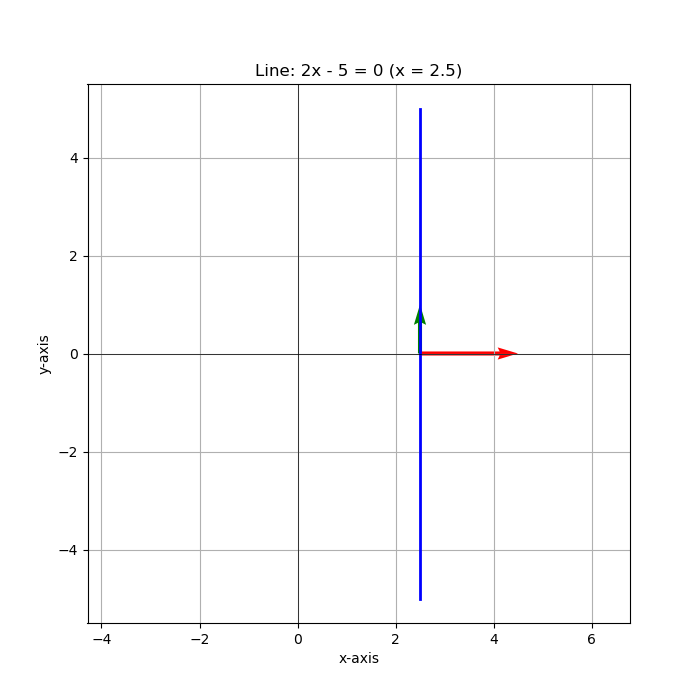
\includegraphics[width=0.7\columnwidth]{Figs/Figure_1.png}
    \caption{Plot of the line $x = 2.5$}
    \label{Fig_428}
\end{figure}

\end{document}

